\chapter{ローカルデータベースにおける読み出し試験結果検索機能の詳細と処理時間測定}

生産時には、読み出し試験の結果は一つの機関で大量に生じるものである。
4章で述べたように、任意のタイミングで必要な結果を取得できる検索機能を実装した。詳細について以下に示す。


\section{実装方法}
今回の実装では、一般的にウェブで用いられているフリーワードの検索エンジンのような機能を実装しようと考えた。
ユーザの操作を最小限にし、柔軟な検索ができるようにするためである。

読み出し試験において、対象とする検索キーワードを以下の項目に絞った。
システムにおいて、アップロードされた試験結果に関わるデータベース内の情報は固定されていて、試験結果情報の変更はしないことを前提としている。
そのため、ユーザが対象としたい検索キーワードは以下の項目に限られ、検索キーワードとして以下の項目をサポートすれば十分であると考えた。

\begin{itemize}
  \item モジュール及びFEチップのID
  \item 読み出し試験項目(例:std$\_$digitalscan)
  \item 読み出し試験者
  \item 読み出し試験場所
  \item 試験日時(将来的に範囲指定を用いた検索機能を検討)
  \item タグ機能を用いてつけられたタグ
\end{itemize}

そこで実装方法として、以下の2つを考えた。

\begin{enumerate}
  \item 各試験に関する情報をPythonリスト集め、検索キーワードが含まれるかを確認する方法
  \item 各試験に関する情報を持つドキュメント、コレクションを予め作成、それを参照し検索を行う方法
\end{enumerate}

これらについて以下で詳細を説明する。

\subsection{方法1: Pythonリストを用いた一致確認}
Pythonリストを使う実装の場合、以下のような流れで検索処理を行う。
\begin{enumerate}
  \item ユーザが検索ワードを入力し、処理を実行
  \item 読み出し試験に関する情報を全て取得
  \item Pythonリストに保持、検索ワード一致を確認、試験を選別
  \item ブラウザーに送信
\end{enumerate}

アルゴリズムのイメージを図\ref{search_python_list}に示す。
この方法では、データベース内の試験結果とアプリケーションの関数内だけで全ての処理を行うことが可能なため、シンプルな実装方法である。

\begin{figure}[bpt]
  \begin{center}
    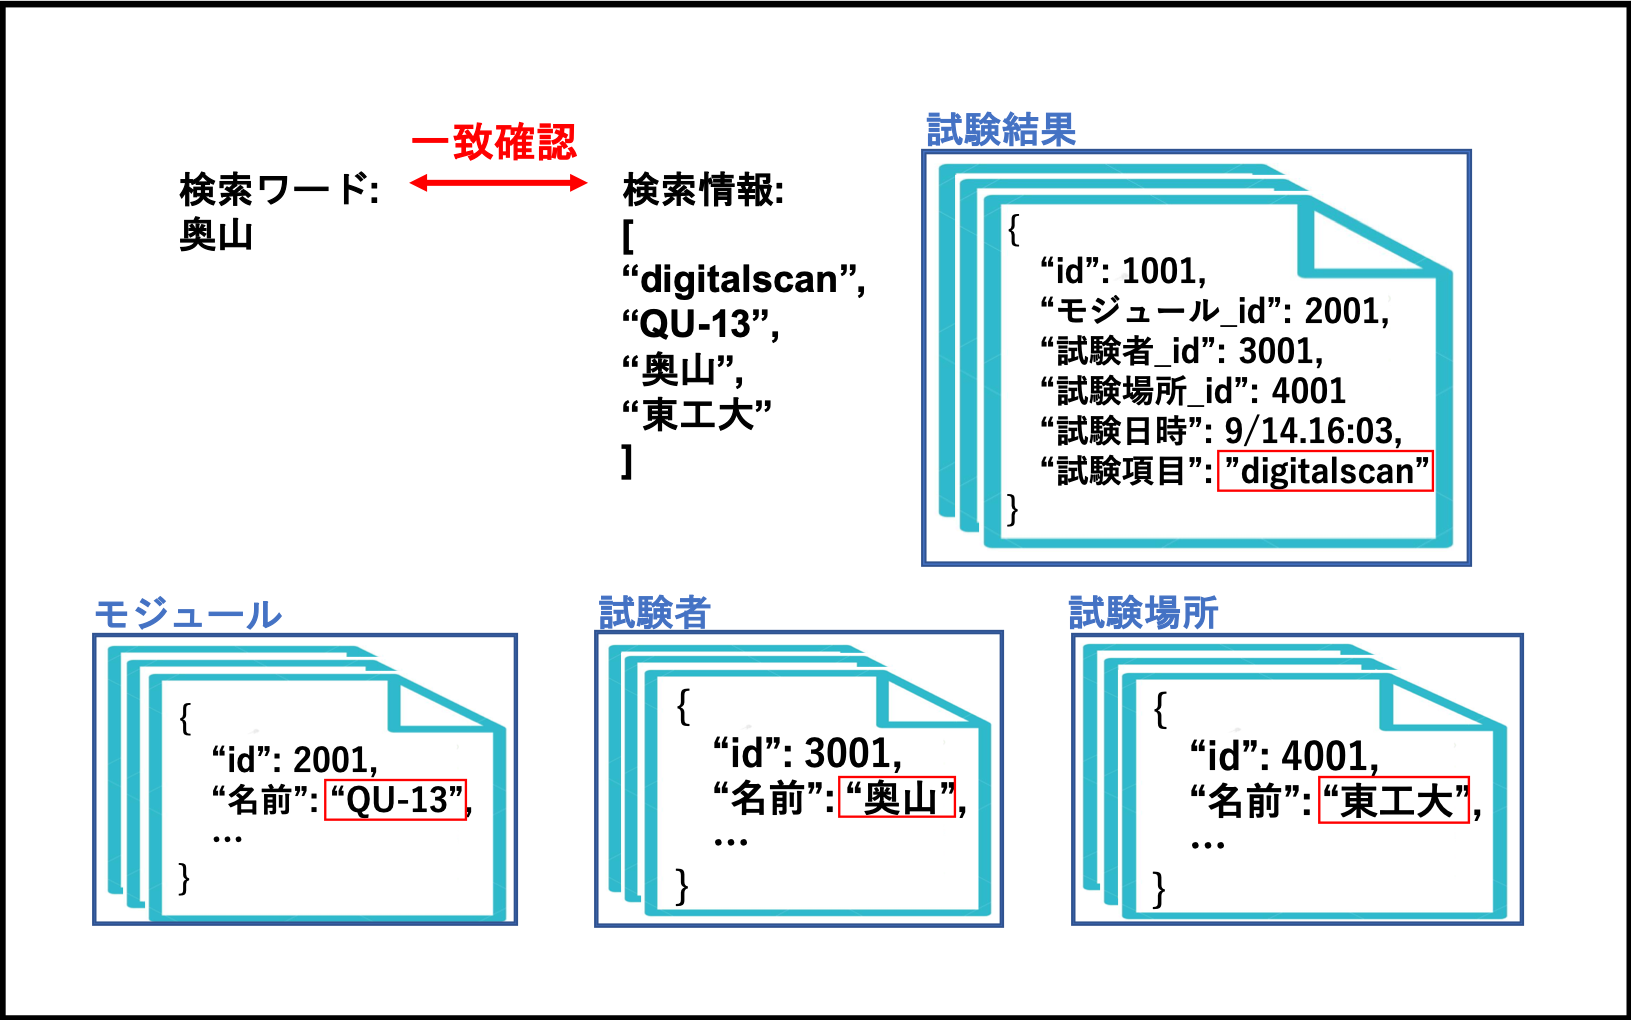
\includegraphics[width=14cm]{search_python_list}
    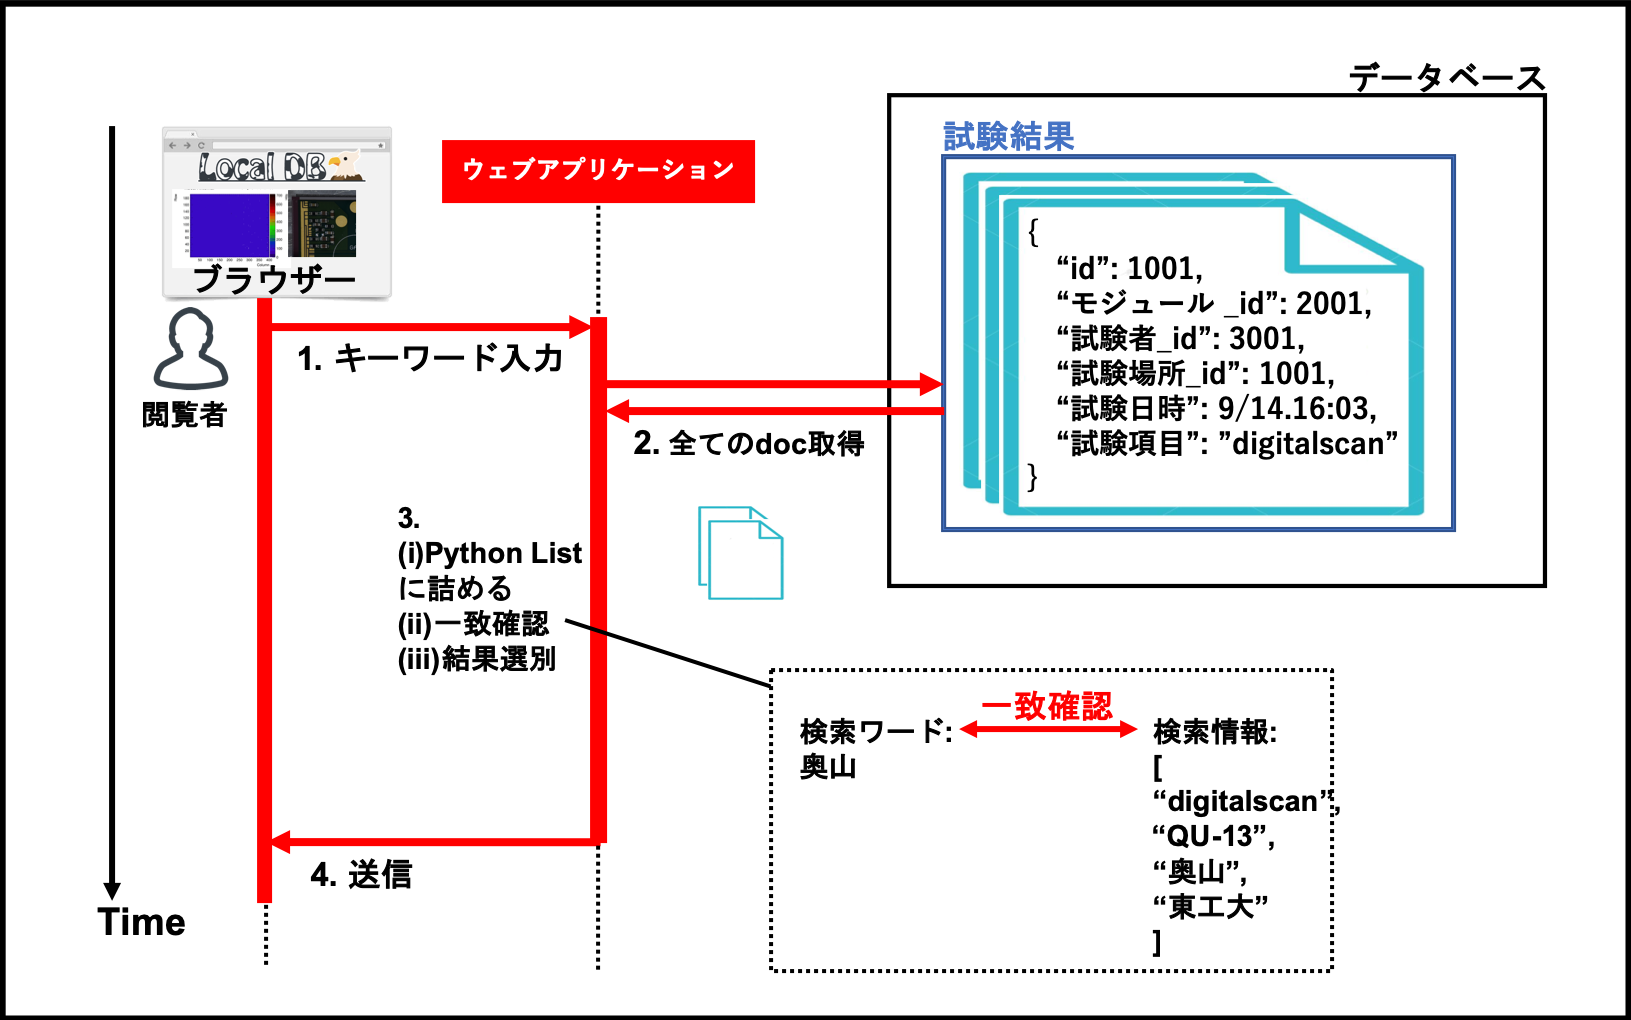
\includegraphics[width=14cm]{search_python_list_flow}
  \caption[検索機能実装方法1:Pythonリストを用いた場合]{検索機能実装方法1:Pythonリストを用いた場合}
  \label{search_python_list}
  \end{center}
\end{figure}

ユーザが処理を実行した際にデータベース内で情報を取得し、Pythonリストにつめる処理を行う。
\\

しかしこの方法を試験実装したところ、データベース内の構造は複雑であり複数のコレクションを跨いで情報を保持しているため、試験結果全てに対してリアルタイムでこの処理を行うと、時間を大きく要してしまう問題が発生した。
イメージを図\ref{search_python_list_problem}に示す。

このシステムにおいては試験結果数を$n$とすると、試験結果情報を保存しているtestRun、componentとtestRunの関係を保存するcomponentTestRunがぞれぞれ$O(n)$のドキュメント数を持つことになる。
各componentの情報を取得し、一致確認を行うと$O(n^2)$の時間がかかる。イメージを図\ref{search_python_testRun}に示す。


\begin{figure}[bpt]
  \begin{center}
    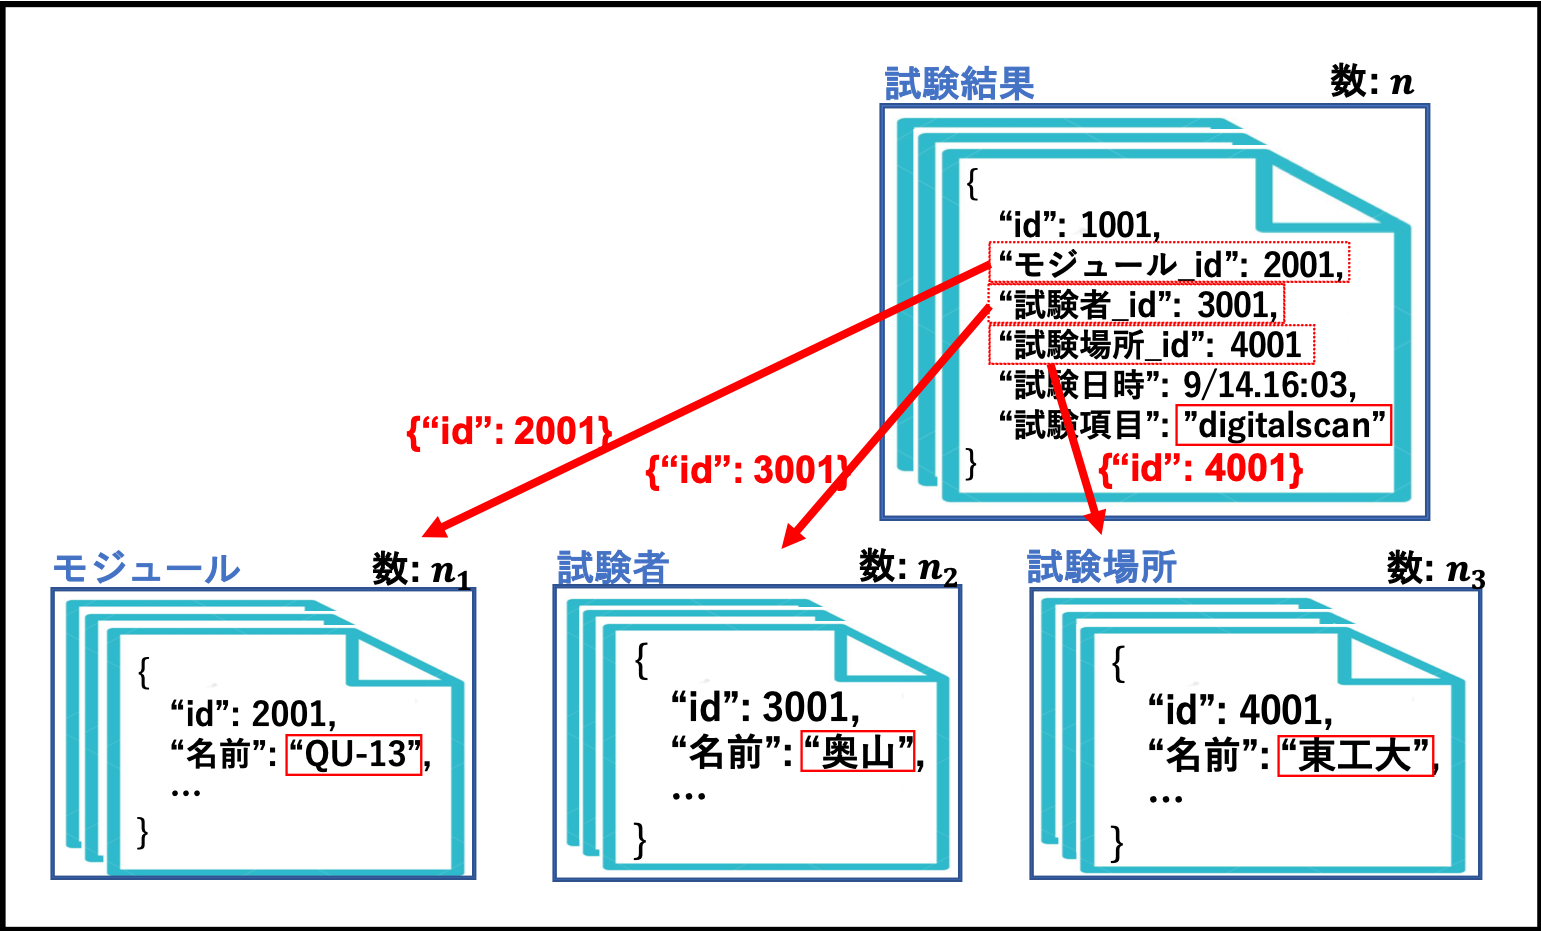
\includegraphics[width=14cm]{search_python_list_problem}
  \caption[検索機能実装方法1の問題点]{検索機能実装方法1の問題点}
  \label{search_python_list_problem}
  \end{center}
\end{figure}

\begin{figure}[bpt]
  \begin{center}
    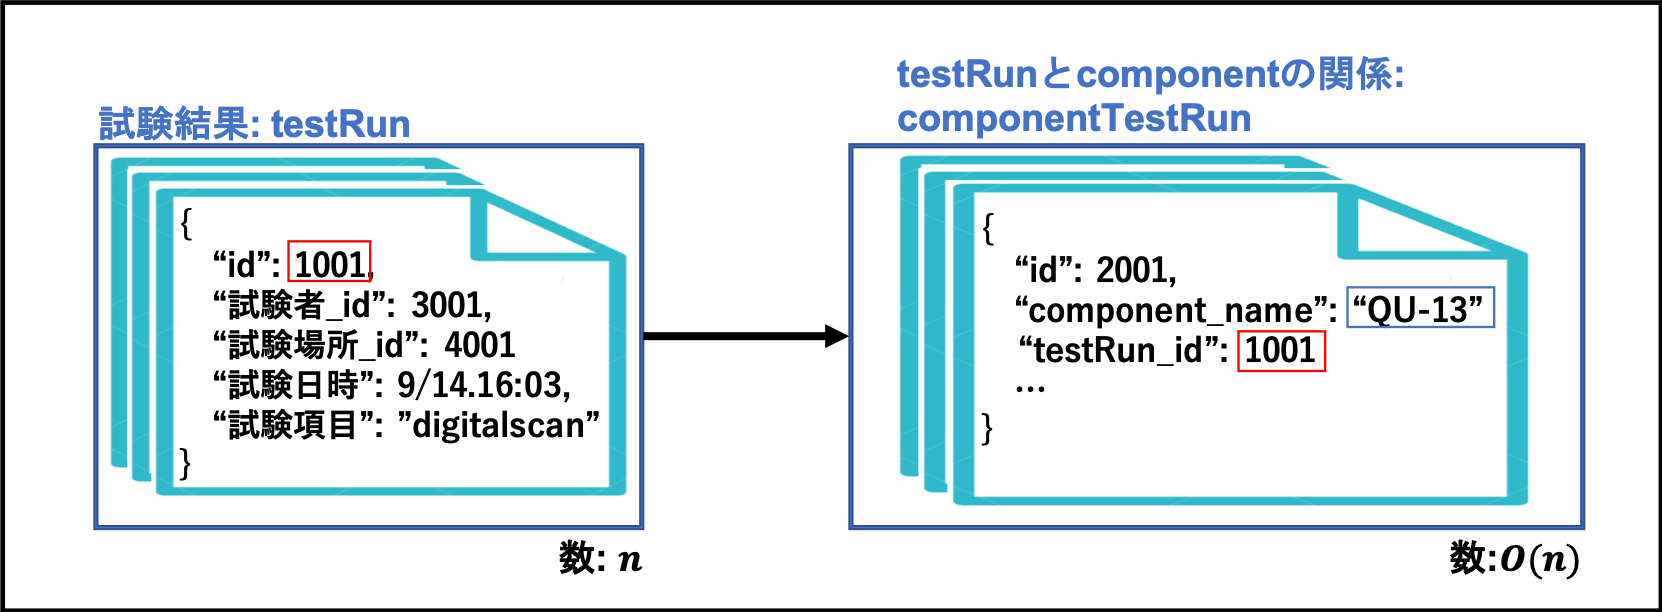
\includegraphics[width=14cm]{search_python_testRun}
  \caption[検索機能実装方法1の問題点詳細]{検索機能実装方法1の問題点詳細}
  \label{search_python_testRun}
  \end{center}
\end{figure}

\subsection{方法2: 検索情報を持つドキュメントを作成、使用}
検索機能を改善するため方法2を考案し、実装を行った。アルゴリズムのイメージを図\ref{search_mongo_collection}に示す。
検索キーワードを別のドキュメントに予め保持しておき、処理実行時にはそれを参照することで検索を行う。
検索情報コレクションに入るドキュメント数は、試験結果数と同じであるため$O(n)$であり、検索コストを削減できると考えた。

\begin{figure}[bpt]
  \begin{center}
    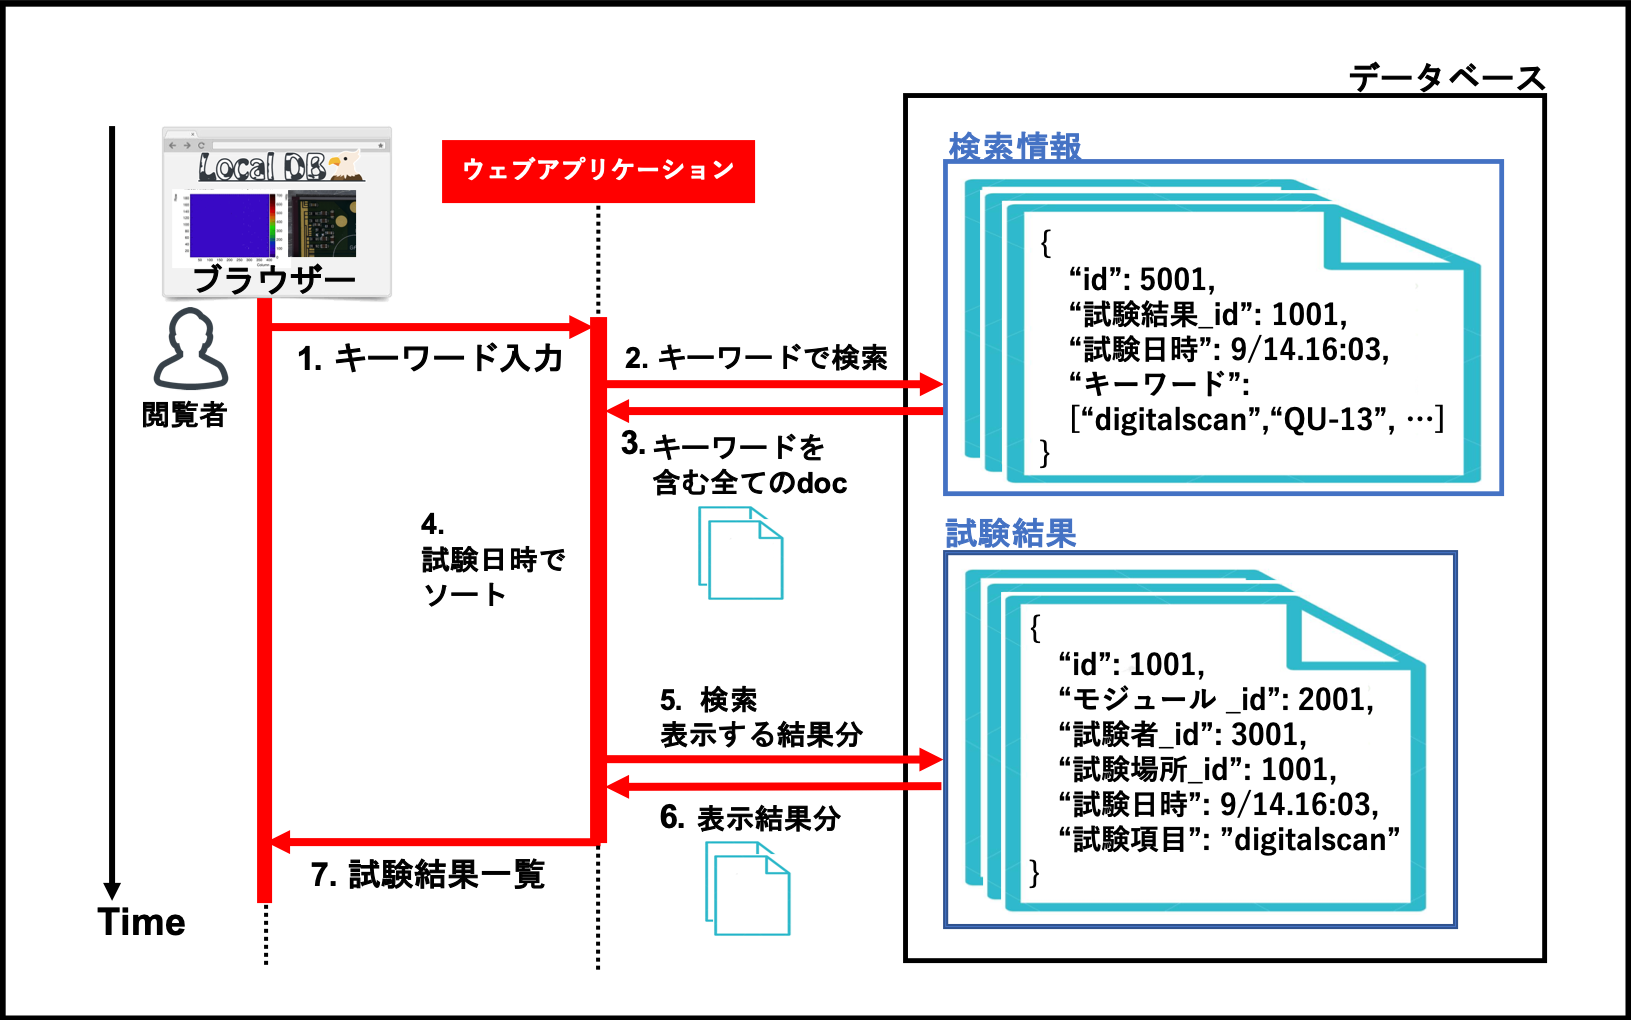
\includegraphics[width=14cm]{search_mongo_collection}
    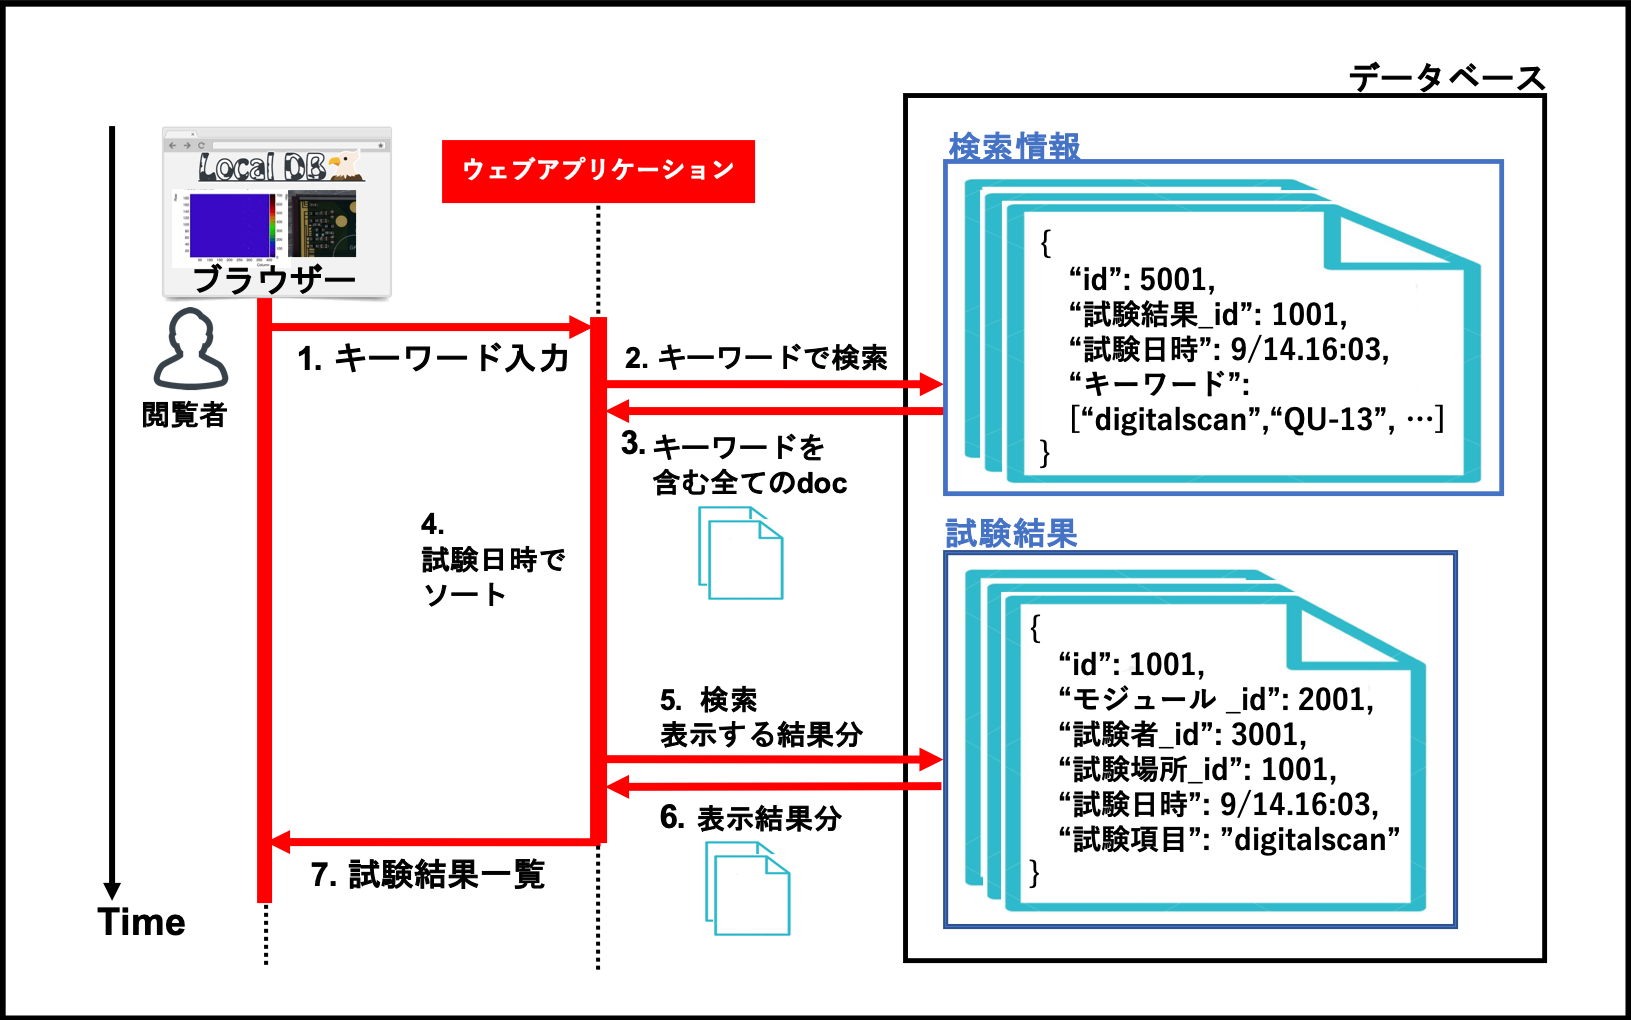
\includegraphics[width=14cm]{search_mongo_collection_flow}
  \caption[検索機能実装方法2:検索キーワード専用コレクションを用いた場合]{検索機能実装方法2:検索キーワード専用コレクションを用いた場合}
  \label{search_mongo_collection}
  \end{center}
\end{figure}

\section{処理時間測定} \label{sec:search_process_time_mes}
先述した方法1と2において、検索処理時間の測定を行った。詳細を以下に示す。


\subsubsection{使用したデバイス}

測定には個人で使用しているノートPC(MacBookAir(13-inch,2017))を用いた。性能を表\ref{laptop_spec}に示す。

\begin{table}[tbp]
\caption[ノートPCの性能]{ノートPCの性能}
\label{laptop_spec}
\scalebox{0.9}{
  \begin{tabular}{|l|llll|l|l|} \hline
    PC名 & CPU & & & & Memory & Disk \\
     & Type & Core & Thread & Clock speed[GHz]& [GB] & [GB] \\ \hline 
    MacBookAir(13-inch,2017) & Intel Core i5 & 2 & 4 & 1.8 & 8 & 256\\ \hline
  \end{tabular}
}
\end{table}


\subsubsection{測定内容}

コマンドプロンプトから以下を使用し、リクエストに対するアプリケーションのレスポンス時間を測定した。
実際にアプリケーションを使用する際には、ブラウザーに一覧表示をする時間が今回の測定時間に加算されることになる。

\begin{lstlisting}
curl "http://127.0.0.1:5000/localdb/scan?keywords=okuyama&match=partial" 
-o /dev/null -w "$\%${time$\_$total}\n" 2> /dev/null -s
\end{lstlisting}

上記のコマンドを用いて、試験結果数に対するレスポンス時間の測定を行った。
測定に関する詳細を表\ref{searching_measurement_details}に示す。

\begin{table}[tbp]
\begin{center}
\caption[検索機能処理時間測定の詳細]{検索機能処理時間測定の詳細}
\label{searching_measurement_details}
\scalebox{0.9}{
  \begin{tabular}{|l|l|} \hline
    試験結果数 & 1, 5000, 10000, 15000, 20000\\
    測定回数 & 各測定点に対して20回\\
    検索キーワード & okuyama\\
    検索モード & 部分一致\\
    各試験結果が持つ検索情報 & 全試験結果に対して同じ、以下に詳細\\\hline
    検索情報一覧             & モジュール名: 20UPGR10000005\\
		                         & FEチップ名:   20UPGTU9000000\\
		                         & 試験項目:     std$\_$digitalscan\\
		                         & 試験者:       okuyama\\
		                         & 試験場所:     default$\_$host\\
		                         & 試験日時:     2020/12/06\\\hline
  \end{tabular}
}
\end{center}
\end{table}


各測定点に対して平均値、標準偏差を算出し、フィッティングを行った。


\subsubsection{測定結果}

結果を図\ref{searching_time}に示す。
また得られた近似関数をそれぞれ式\ref{function_python_list}、\ref{function_mongo_collection}に示す。
方法1に対して、方法2の処理時間は改善されていることが分かる。

\begin{figure}[bpt]
  \begin{center}
  \begin{minipage}{0.4\hsize}
    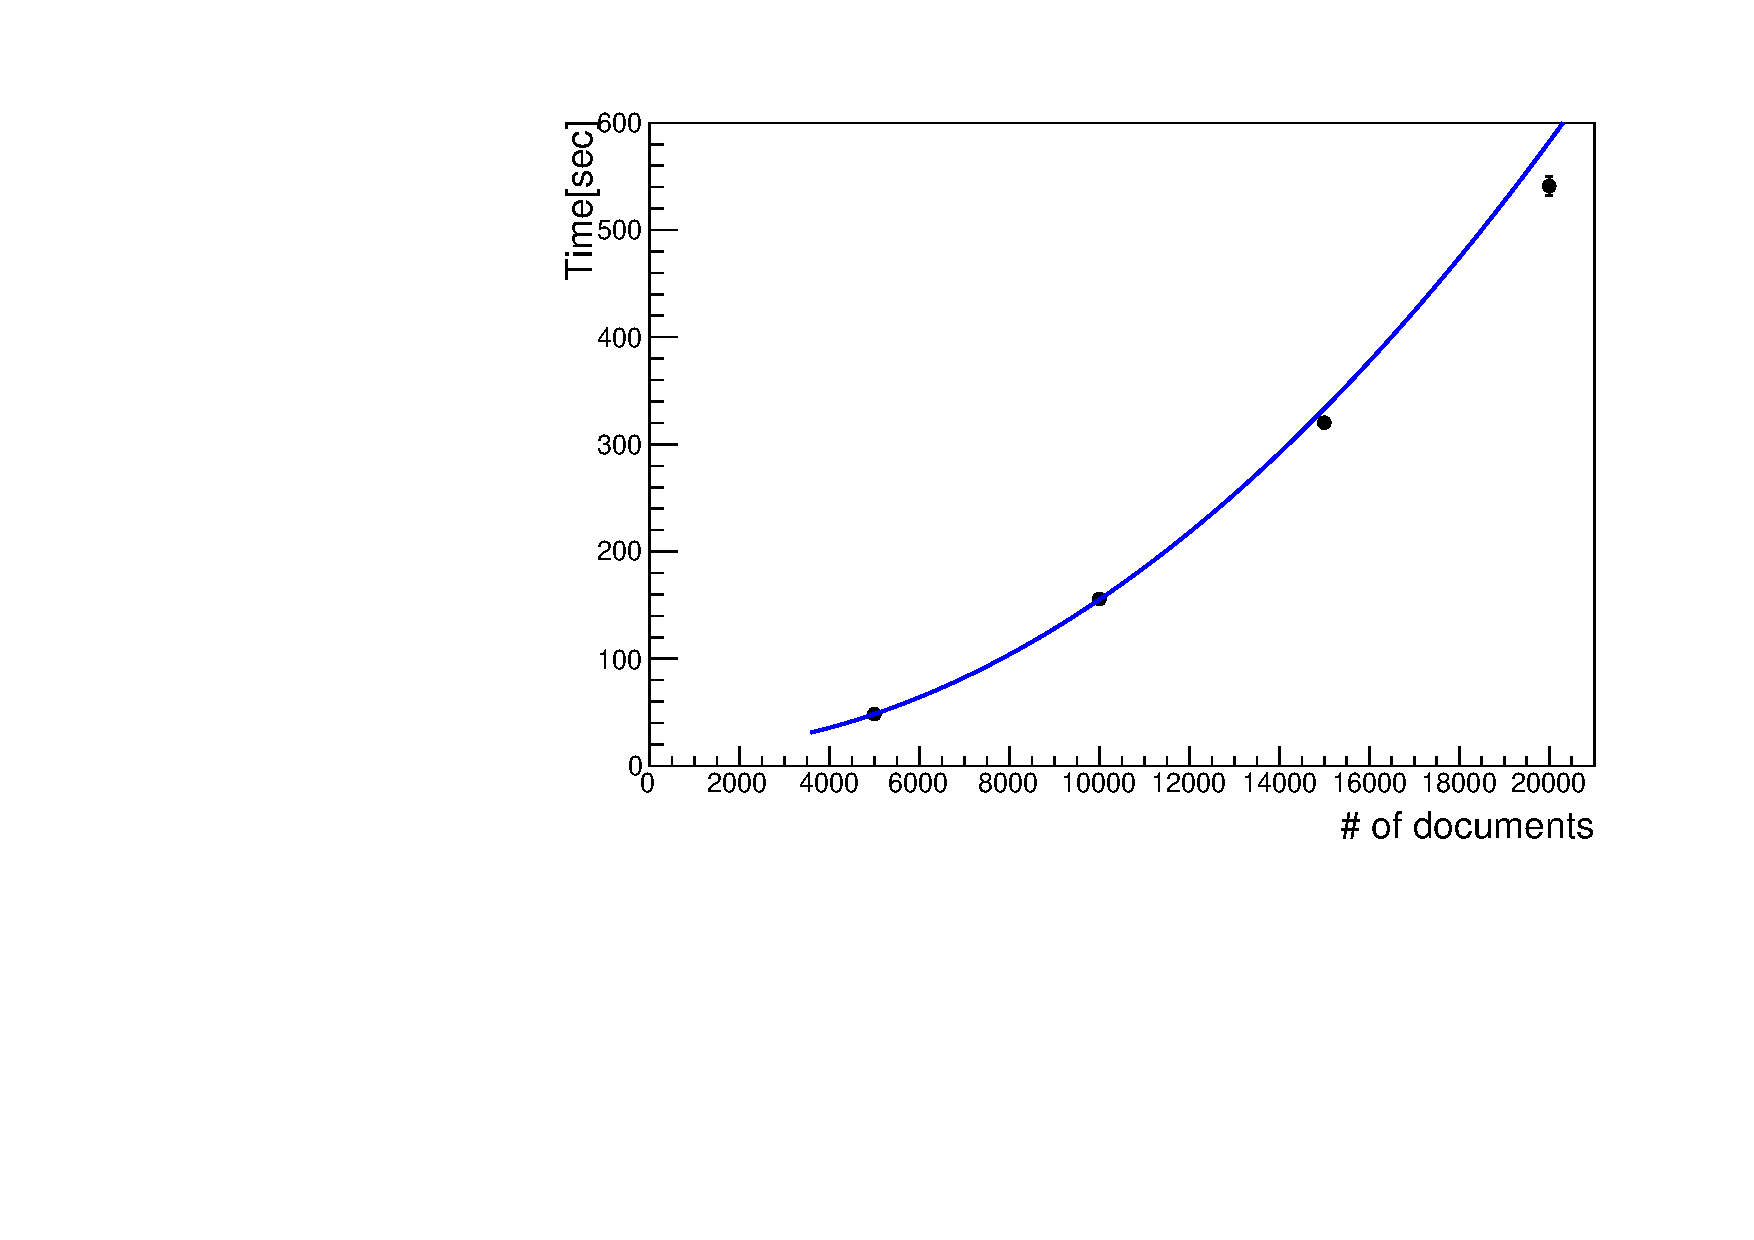
\includegraphics[width=4cm,angle=270]{result_python_list_search.pdf}
  \end{minipage}
  \begin{minipage}{0.4\hsize}
    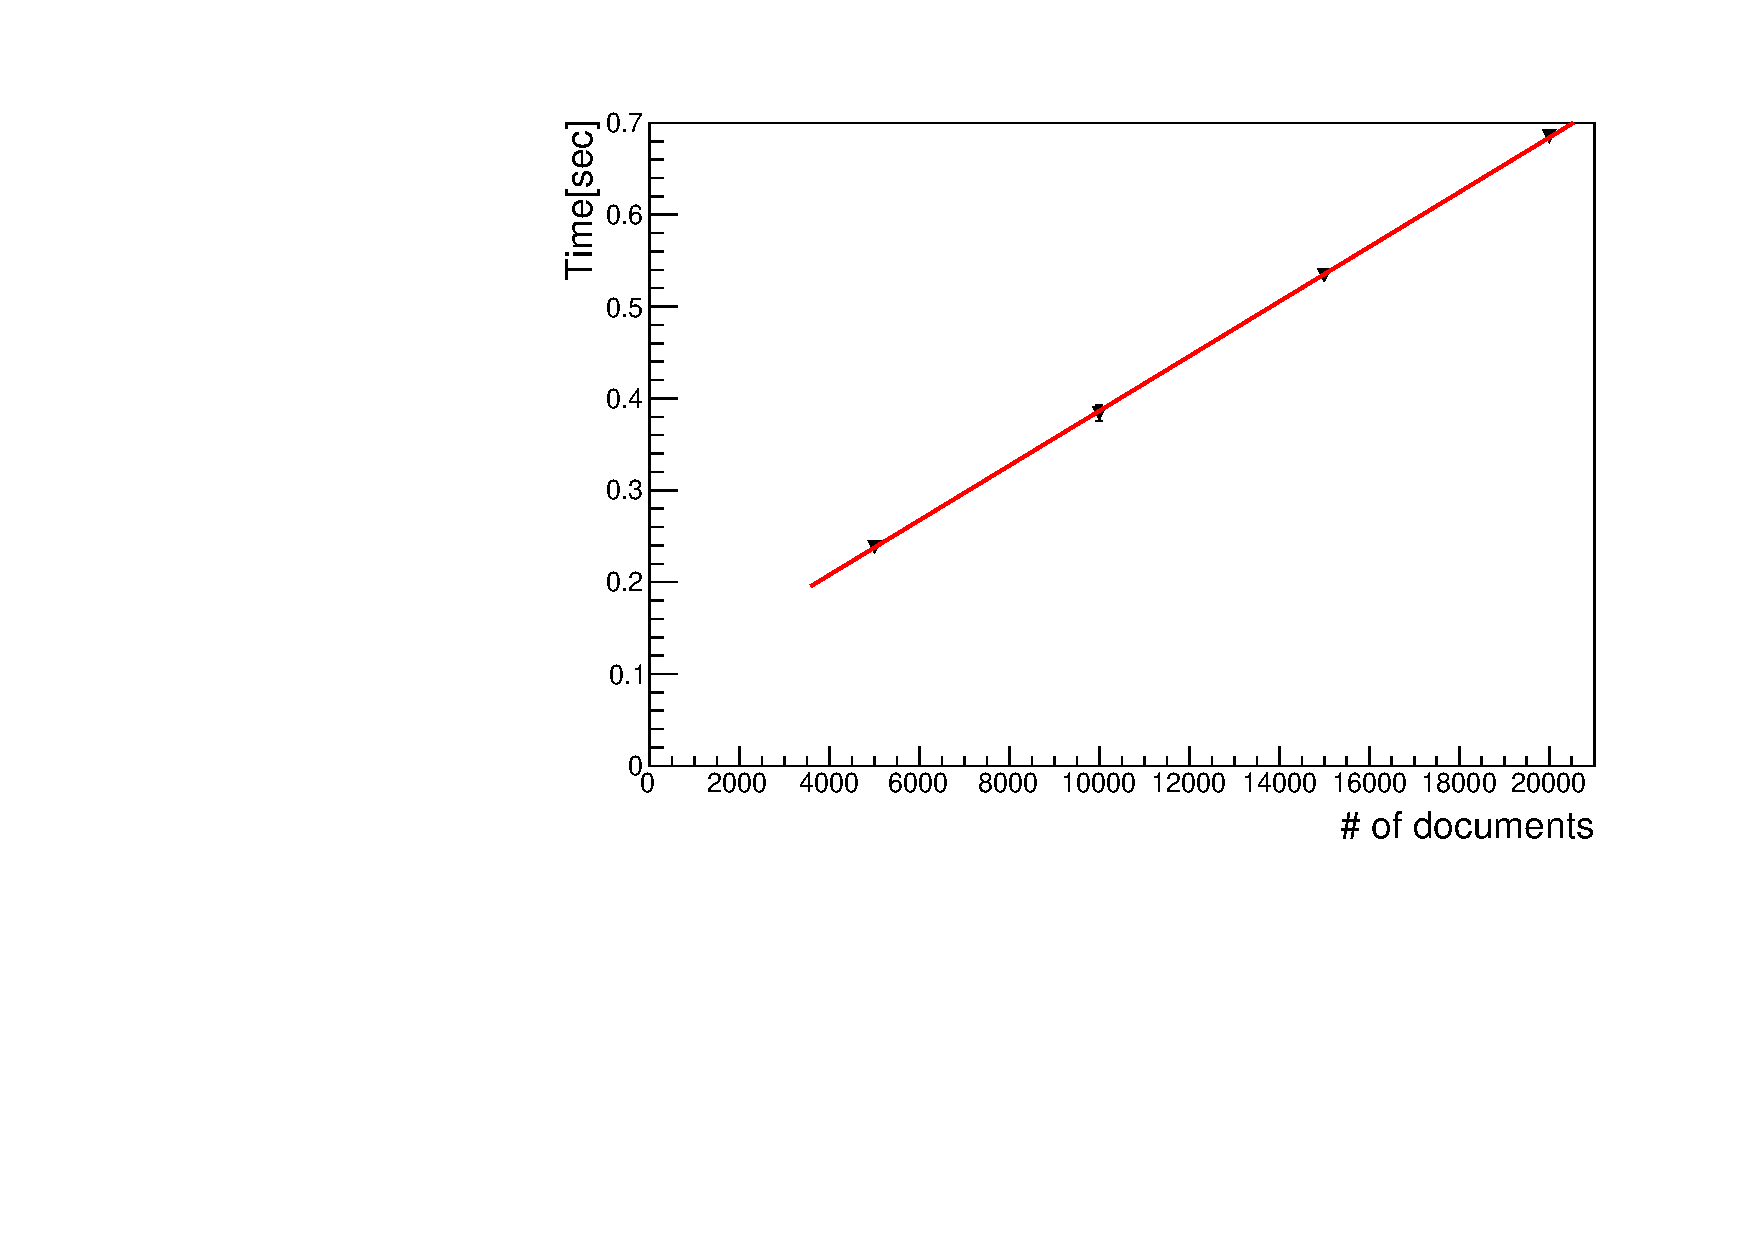
\includegraphics[width=4cm,angle=270]{result_mongo_collection_search.pdf}
  \end{minipage}

  \caption[検索処理速度測定]{検索処理速度測定}
  \label{searching_time}
  \end{center}
\end{figure}

\bbb
y =  \{(1.4\pm0.0)\times10^{-6}\}x^2 + (13\pm 0)
\label{function_python_list}
\eee
\bbb
y = \{(3.0\pm0.1)\times10^{-5}\}x + \{(8.9\pm 0.8)\times10^{-2}\}
\label{function_mongo_collection}
\eee

現在は方法2で検索機能を実装し、サービスの1つとして提供している。

\subsubsection{生産時における検索時間の見積もり}
各方法について、生産時における処理時間の見積もりを行う。簡単のため今回使用したデバイスと生産時に使うサーバーの性能差は無視する。
ここでデータベースで管理するモジュール数は日本が最多とし、その数を予定している2,000とする。
保存する読み出し試験数は3章で述べたように、1つのモジュールあたり42とする。全ての生産が終了した際の検索処理時間を見積もる。
上で得られた関係式を用いて検索処理実行時間は方法1、2に対して式\ref{estimated_python_list}、\ref{estimated_mongo_collection}のように見積もることができる。

\bbb
\{(1.4\pm0.0)\times10^{-6}\}\times(2000\times42)^2 + (13\pm 0) = (9.8\pm0)\times10^{3} [\rm{sec}]
\label{estimated_python_list}
\eee
\bbb
\{(3.0\pm0.1)\times10^{-5}\}\times(2000\times42) + \{(8.9\pm 0.8)\times10^{-2}\} = 2.6\pm0.1 [\rm{sec}]
\label{estimated_mongo_collection}
\eee

方法1では約9800秒の処理時間が見積もられ、生産時には何台ものモジュール結果の保存、管理をすることから運用不可能である。
方法2では終了時点においても数秒で処理を終えることができるため、生産を通して十分に運用可能であると考えれる。
 
\newpage
\section{処理時間の改善方法の考案と実装}

更なる処理時間の改善を目的として、新たな処理アルゴリズムの考案と測定を行った。詳細について以下に示す。

\subsection{方法2における検索処理時間の内訳}
先述したように、方法2では処理時間が改善した。
この方法2について、処理時間の内訳を知るために追加で測定を行った。
アプリケーション層での各処理について、以下のように番号をつける。
\begin{enumerate}
  \item キーワードを受け取り、検索情報コレクションに検索をかけるまでの処理
  \item 検索情報コレクションに検索をかけ、情報を受け取る処理
  \item ドキュメントを受け取り該当する試験結果のIdをまとめ、検索をかけるまでの処理
  \item 試験結果コレクションに検索をかけ、情報を受け取る処理
  \item ドキュメントを受け取りデータを整形、ブラウザにレスポンスを返すまでの処理
\end{enumerate}

イメージを図\ref{search_mongo_collection_details}に示す。

\begin{figure}[bpt]
  \begin{center}
    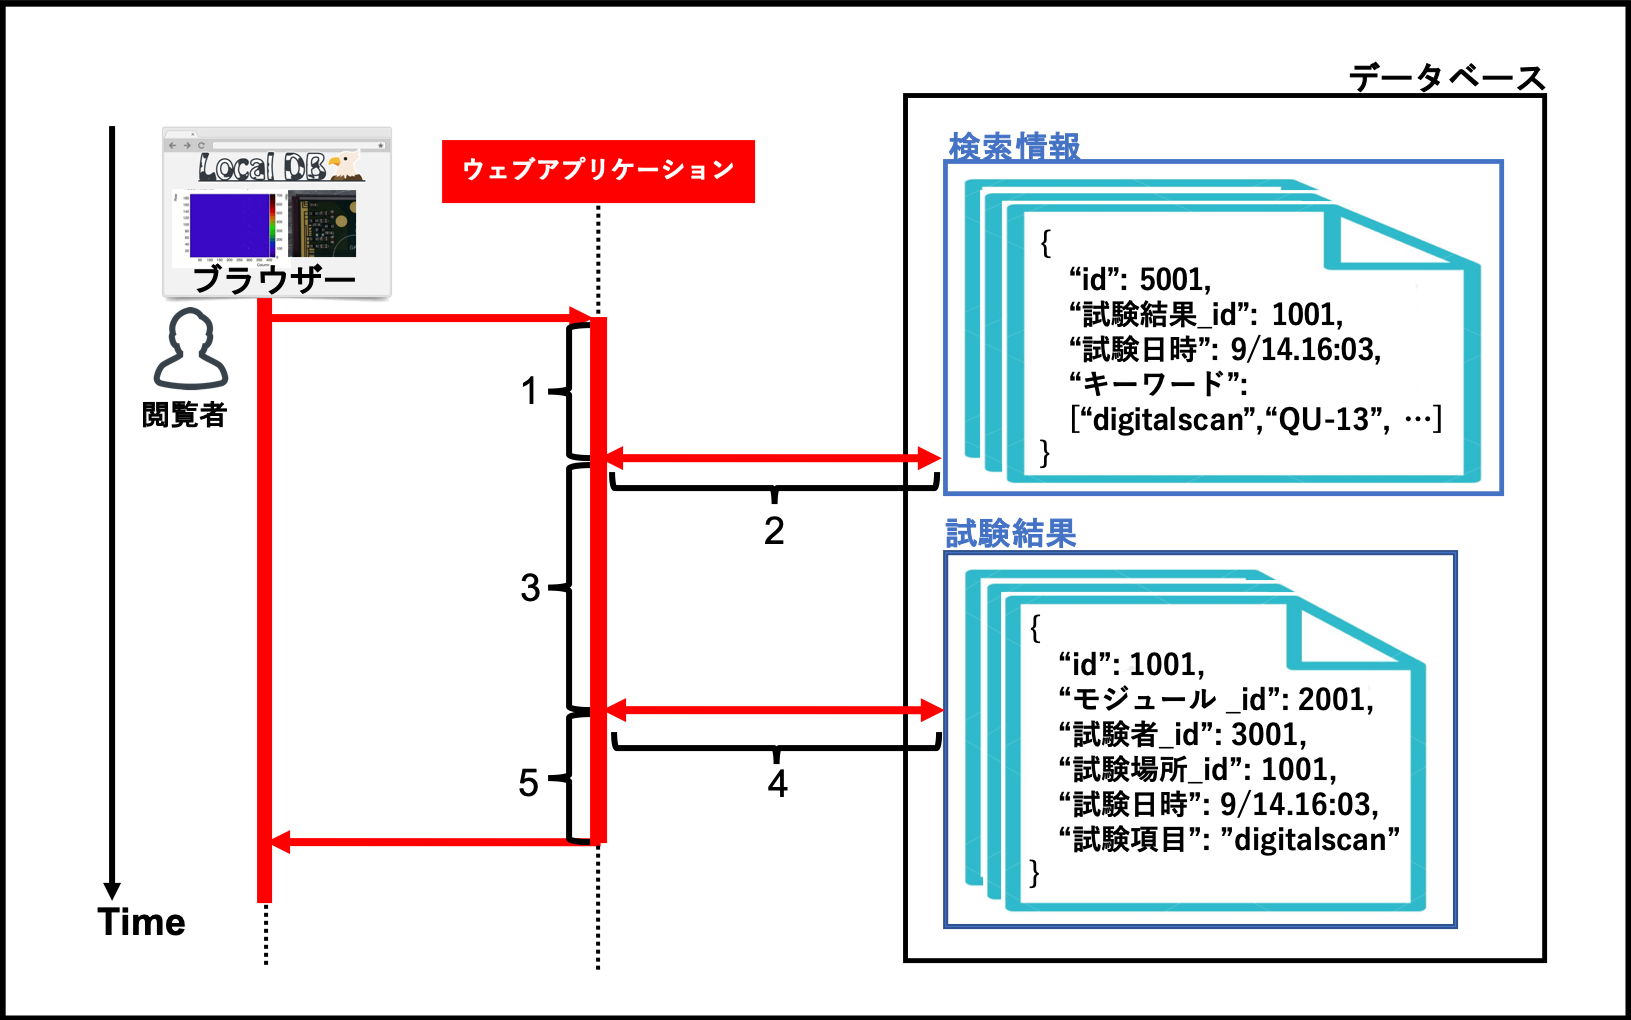
\includegraphics[width=14cm]{search_mongo_collection_details}
  \caption[方法2における検索処理詳細]{方法2における検索処理詳細}
  \label{search_mongo_collection_details}
  \end{center}
\end{figure}

ボトルネックとなっている処理を測定するために、各処理にかかる時間の測定を行った。
測定に関しての詳細を表\ref{search_mongo_collection_details_measurement}に示す。

\begin{table}[tbp]
\begin{center}
\caption[検索機能処理時間測定の詳細]{検索機能処理時間測定の詳細}
\label{search_mongo_collection_details_measurement}
\scalebox{0.9}{
  \begin{tabular}{|l|l|} \hline
    試験結果数 & 10000\\
    測定回数 & 20回\\\hline
  \end{tabular}
}
\end{center}
\end{table}

結果を図\ref{search_mongo_collection_details_result}に示す。

\begin{figure}[bpt]
  \begin{center}
    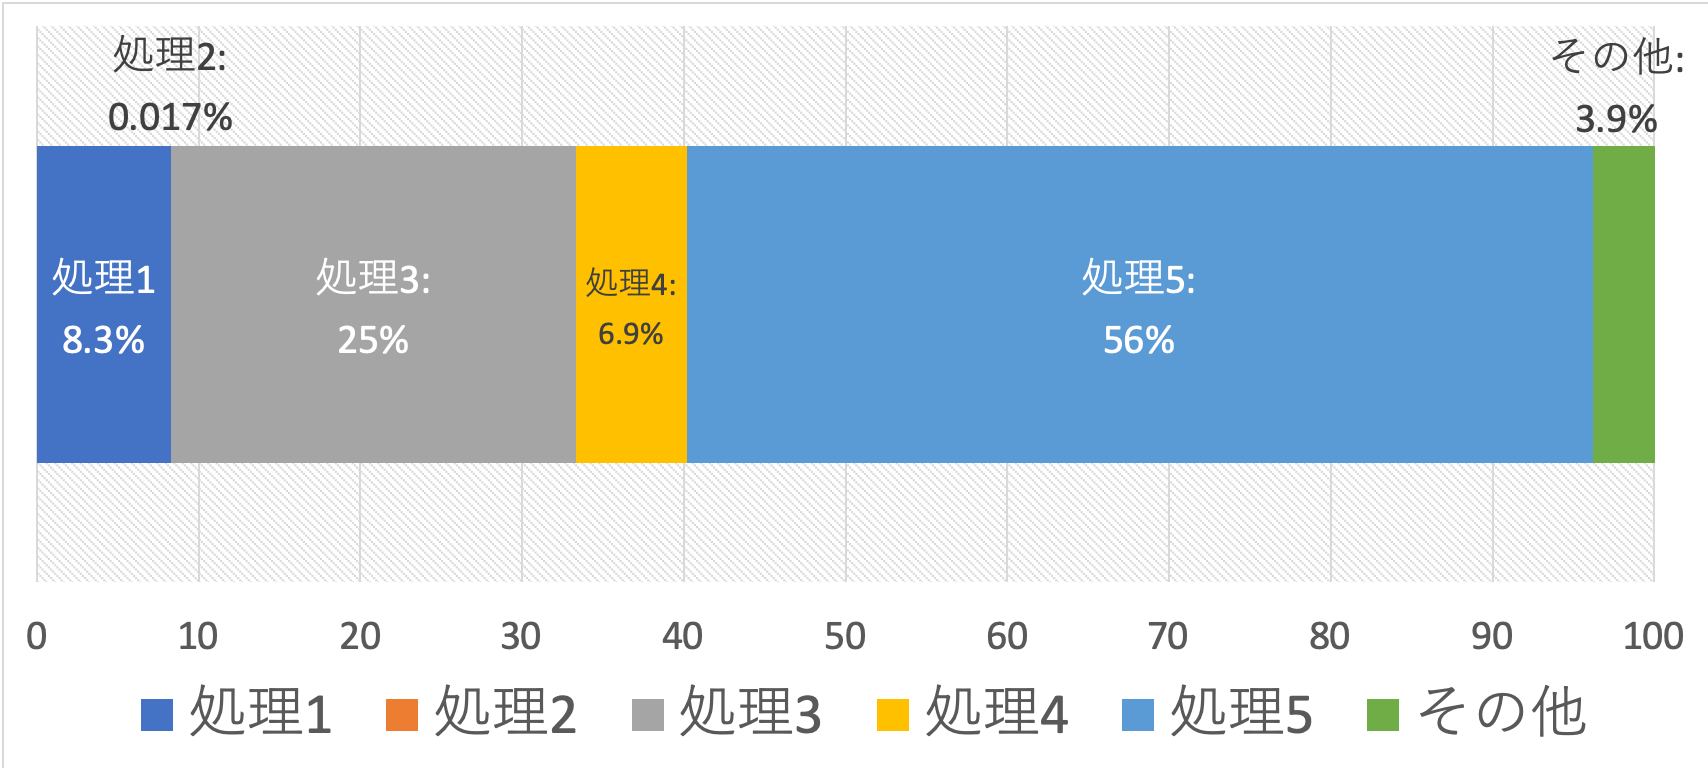
\includegraphics[width=14cm]{search_mongo_collection_details_result}
  \caption[方法2における検索処理詳細結果]{方法2における検索処理詳細結果}
  \label{search_mongo_collection_details_result}
  \end{center}
\end{figure}

処理3,5の割合が大きいことがわかる。
これらについてさらに内訳を調べたところ、以下の処理の割合が大きいことがわかった。
\bbb
\begin{split}
&取得した複数ドキュメントを\rm{Python}リストに変換する処理&
\label{dominated_process}
\end{split}
\eee

上述した方法2における処理3,5において、処理\ref{dominated_process}の割合を表\ref{ratio_dominated_process}まとめた

\begin{table}[tbp]
\begin{center}
\caption[処理3,5における処理\ref{dominated_process}の割合]{処理3,5における処理\ref{dominated_process}の割合}
\label{ratio_dominated_process}
\scalebox{1.0}{
  \begin{tabular}{|llll|} \hline
    処理 & 全体[sec] & 処理\ref{dominated_process}[sec] & 割合[$\%$]\\\hline
    3    & 0.091 & 0.089 & 97 \\
    5    & 0.21 & 0.18 &  86 \\\hline
  \end{tabular}
}
\end{center}
\end{table}

またある検索時におけるコレクション内部の全ドキュメント数と処理\ref{dominated_process}に要する時間の関係を図\ref{dominated_process_relation}に示す。
全ドキュメント数に対して線形性を示していることがわかる。
\begin{figure}[bpt]
  \begin{center}
    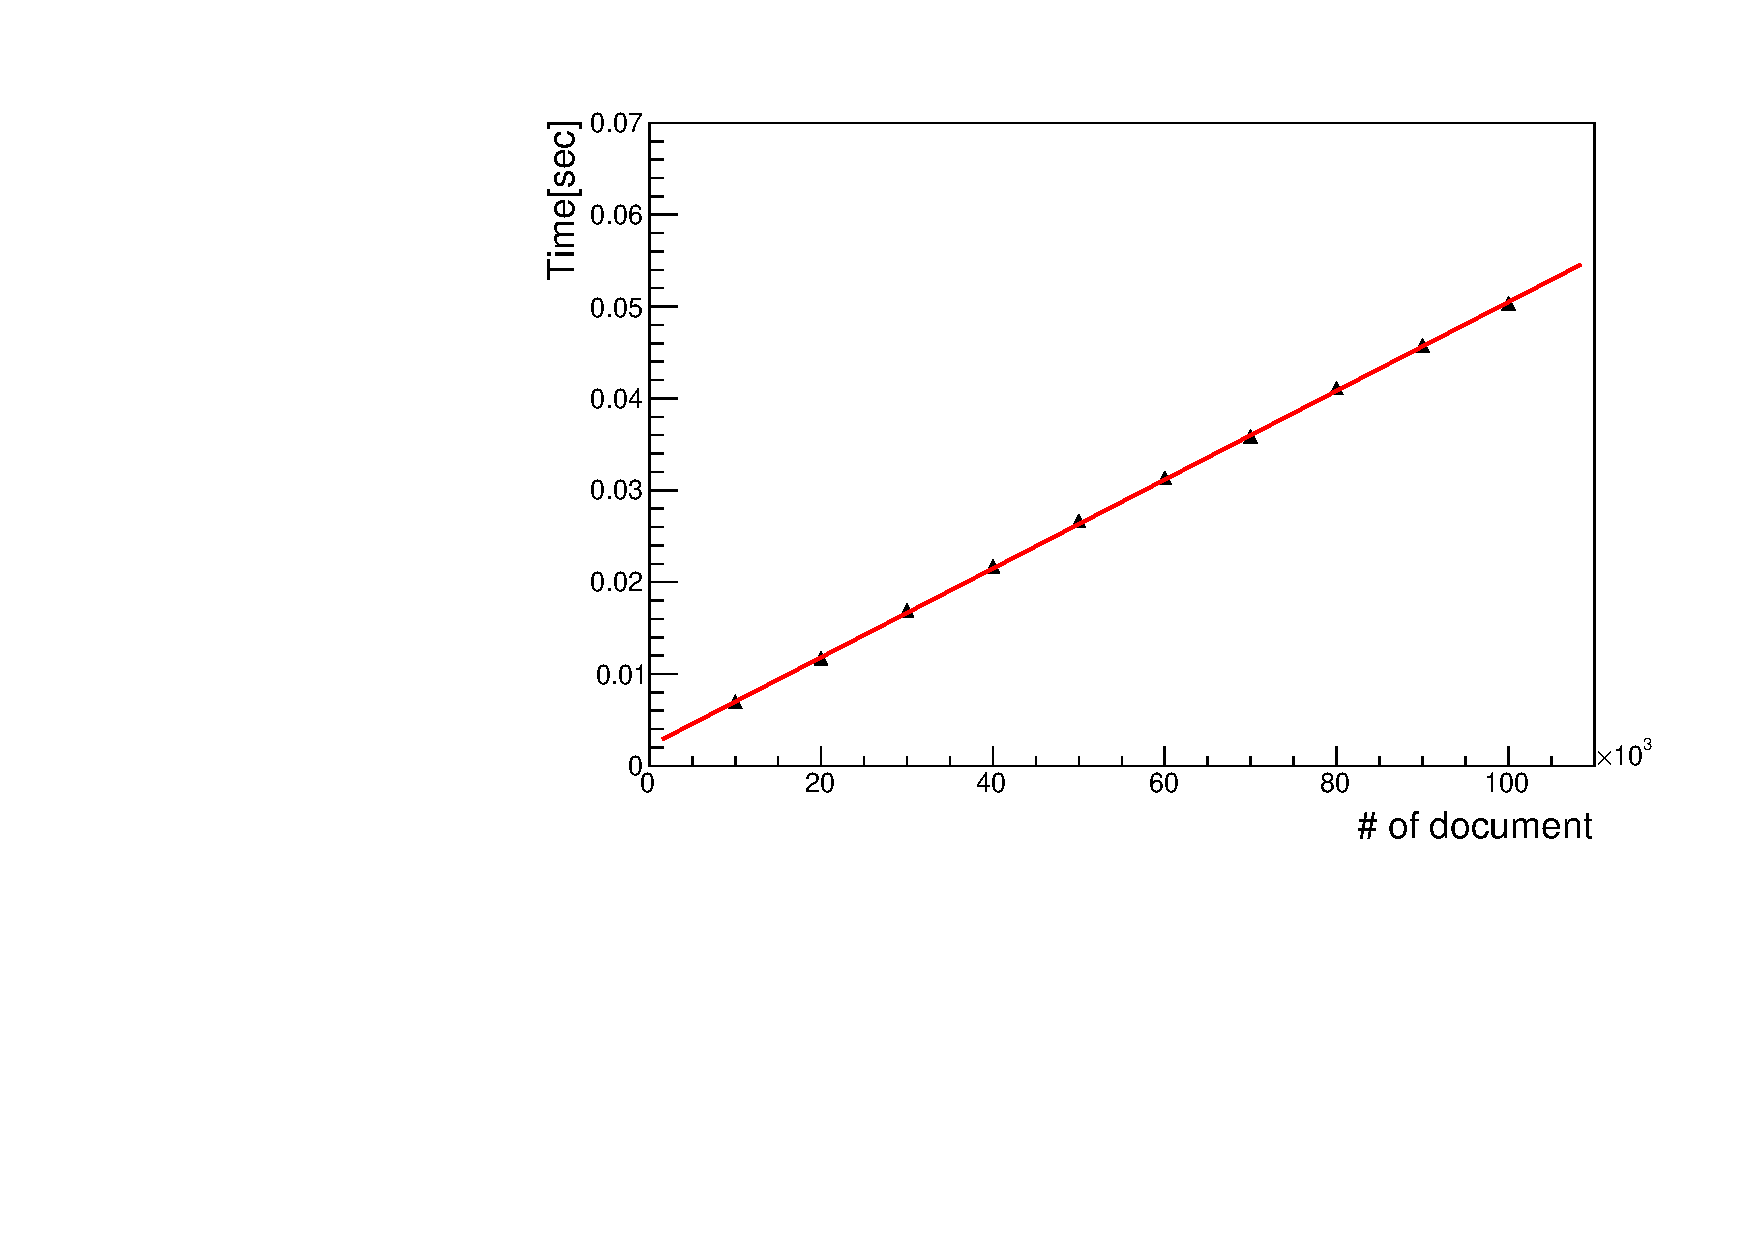
\includegraphics[width=10cm,angle=270]{dominated_process_relation.pdf}
  \caption[ドキュメント数に対するリスト変換処理時間の関係]{ドキュメント数に対するリスト変換処理時間の関係}
  \label{dominated_process_relation}
  \end{center}
\end{figure}

\subsection{改善点}
上記の測定を踏まえ、改善方法として以下の項目を検討した。
\begin{itemize}
  \item 検索処理の回数を減らす
  \item 検索対象コレクションのドキュメント数を減らす
\end{itemize}

上述した2つを目的として、以下の2つの方法を新しく考え処理時間測定を行った。

\begin{enumerate}
  \setcounter{enumi}{2}
  \item 検索情報のコレクションに一覧表示に必要な情報を保持、参照 
  \item 方法3に付け加えて、検索情報のドキュメントを複数コレクションに分散、マルチスレッド
\end{enumerate}

方法3については処理の数を減らし、データベースに対する検索の回数を減らすことを目的としている。
方法4については処理の数を減らすことに加えて、ドキュメントの数を分散し並列処理をすることで処理時間の改善を図っている。
イメージをそれぞれ図\ref{search_summary_hash}、\ref{search_multi_thread}に示す。

\begin{figure}[bpt]
  \begin{center}
    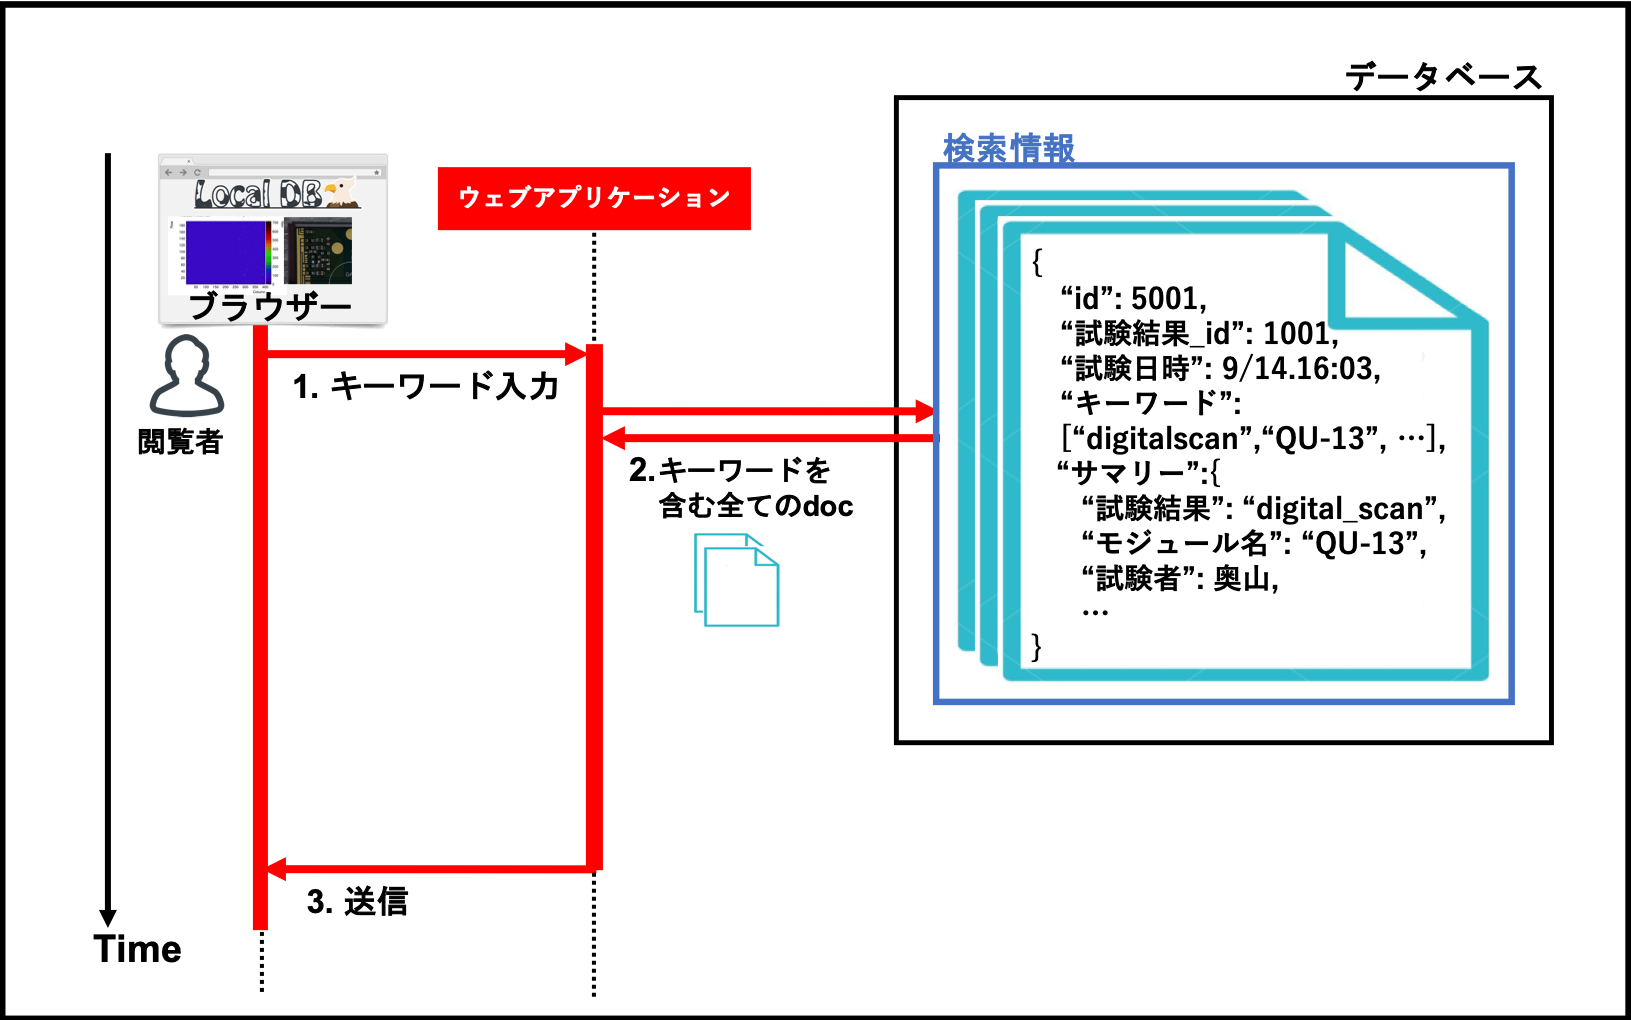
\includegraphics[width=14cm]{search_summary_hash}
  \caption[検索機能実装方法3:検索情報と共に一覧表示に必要な情報を保持]{検索機能実装方法3:検索情報と共に一覧表示に必要な情報を保持}
  \label{search_summary_hash}
  \end{center}
\end{figure}

\begin{figure}[bpt]
  \begin{center}
    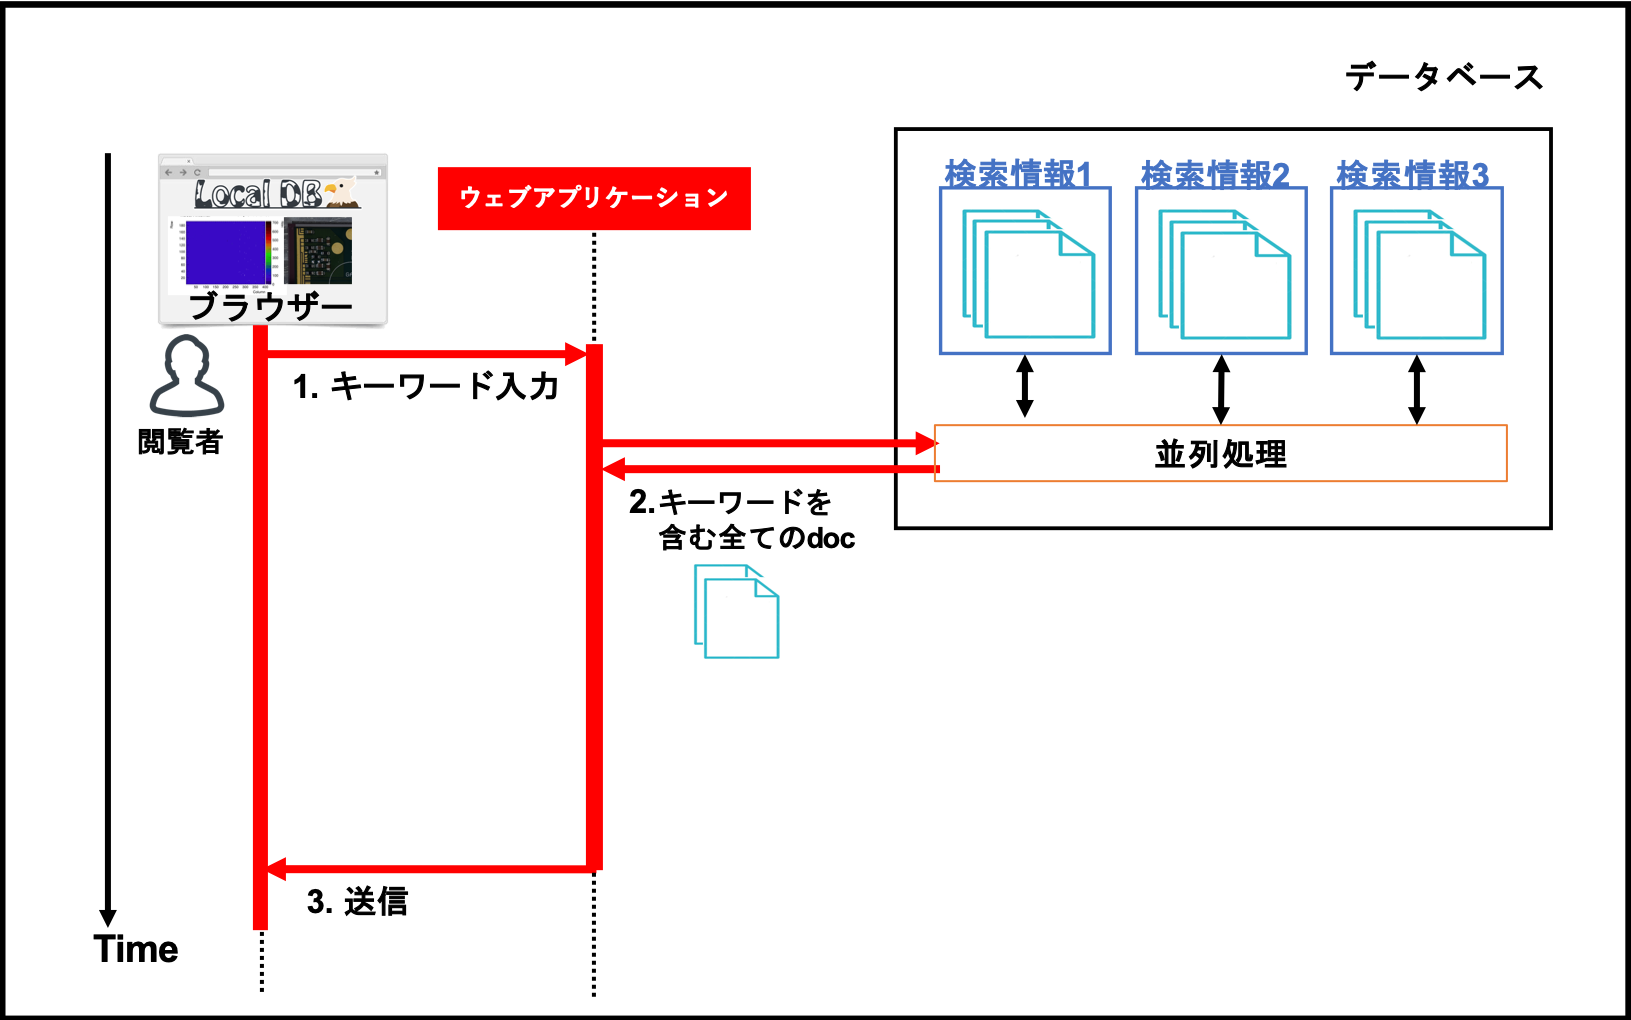
\includegraphics[width=14cm]{search_multi_thread}
  \caption[検索機能実装方法4:検索情報コレクションを分散、マルチスレッドを用いる]{検索機能実装方法4:検索情報コレクションを分散、マルチスレッドを用いる}
  \label{search_multi_thread}
  \end{center}
\end{figure}

方法3,4について、章\ref{sec:search_process_time_mes}と同じ内容の測定を行った。
方法2のものと合わせた結果を\ref{searching_time_2}に示す。
処理時間の改善に成功した。
得られた方法3,4に関する関係を式\ref{function_summary_hash}、\ref{function_multi_thread}に示す。

\begin{figure}[bpt]
  \begin{center}
    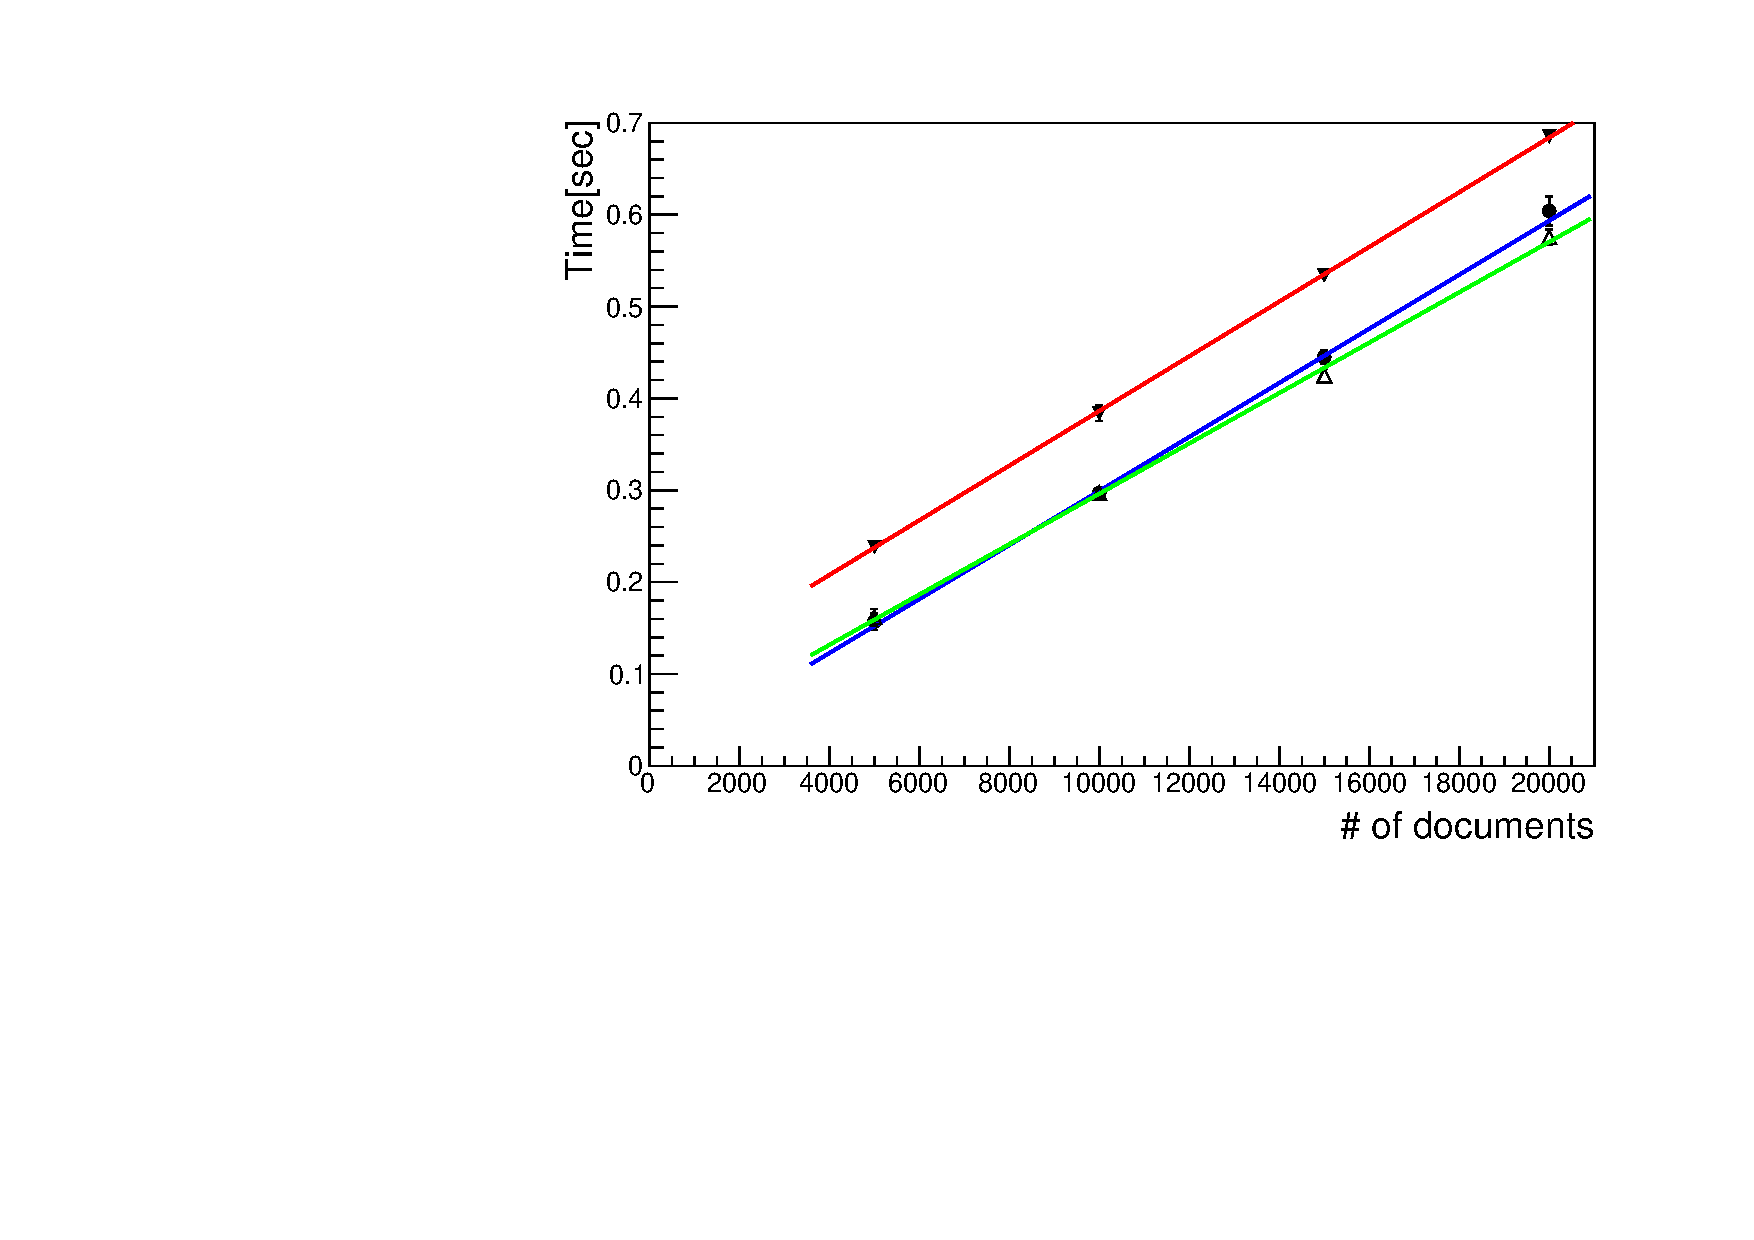
\includegraphics[width=10cm,angle=270]{searching_time_2.pdf}
  \caption[検索機能実装方法3,4に対する測定]{検索機能実装方法3,4に対する測定}
  \label{searching_time_2}
  \end{center}
\end{figure}

\bbb
y = \{(2.9\pm0.1)\times10^{-5}\}x + \{(5.0\pm 11)\times10^{-3}\}
\label{function_summary_hash}
\eee

\bbb
y = \{(2.7\pm0.1)\times10^{-5}\}x + \{(2.2\pm 1.0)\times10^{-2}\}
\label{function_multi_thread}
\eee


